% Compared are tracks ghost associated to the un-groomed large-R jet and the collection used for $\mtas$, see Section \ref{subsec:mtas_def}; ghost association to $k_{\text{t}}$-subjets and $\Delta R$ matching of tracks close to subjets.
Tracks ghost associated to the un-groomed large-$R$ jet and the ones ghost associated to $k_{\text{t}}$-subjets and $\Delta R$ matched with the closest subjets are compared.

The distributions showing the number of tracks associated to a calorimeter jet, see the left side of Figure \ref{fig:delta_R}, indicate, that on average around four tracks less are associated to the subjets compared to the un-groomed jet. The right side of Figure \ref{fig:delta_R} shows the angular distance $\Delta R$ between the single tracks and the axis of the large-R calorimeter jet. Both distributions are aligned in the lower $\Delta R$ region while the histogram representing the tracks associated to the un-groomed jet shows an enhancement towards larger $\Delta R$. Accordingly, the additional tracks feature an angular separation from the jet axis of more than $0.3$. Given the required primary vertex association, it is unlikely that these tracks originate from pile-up. Instead, the origin might be found in final- or initial state radiation. 
\begin{figure}
	\centering
	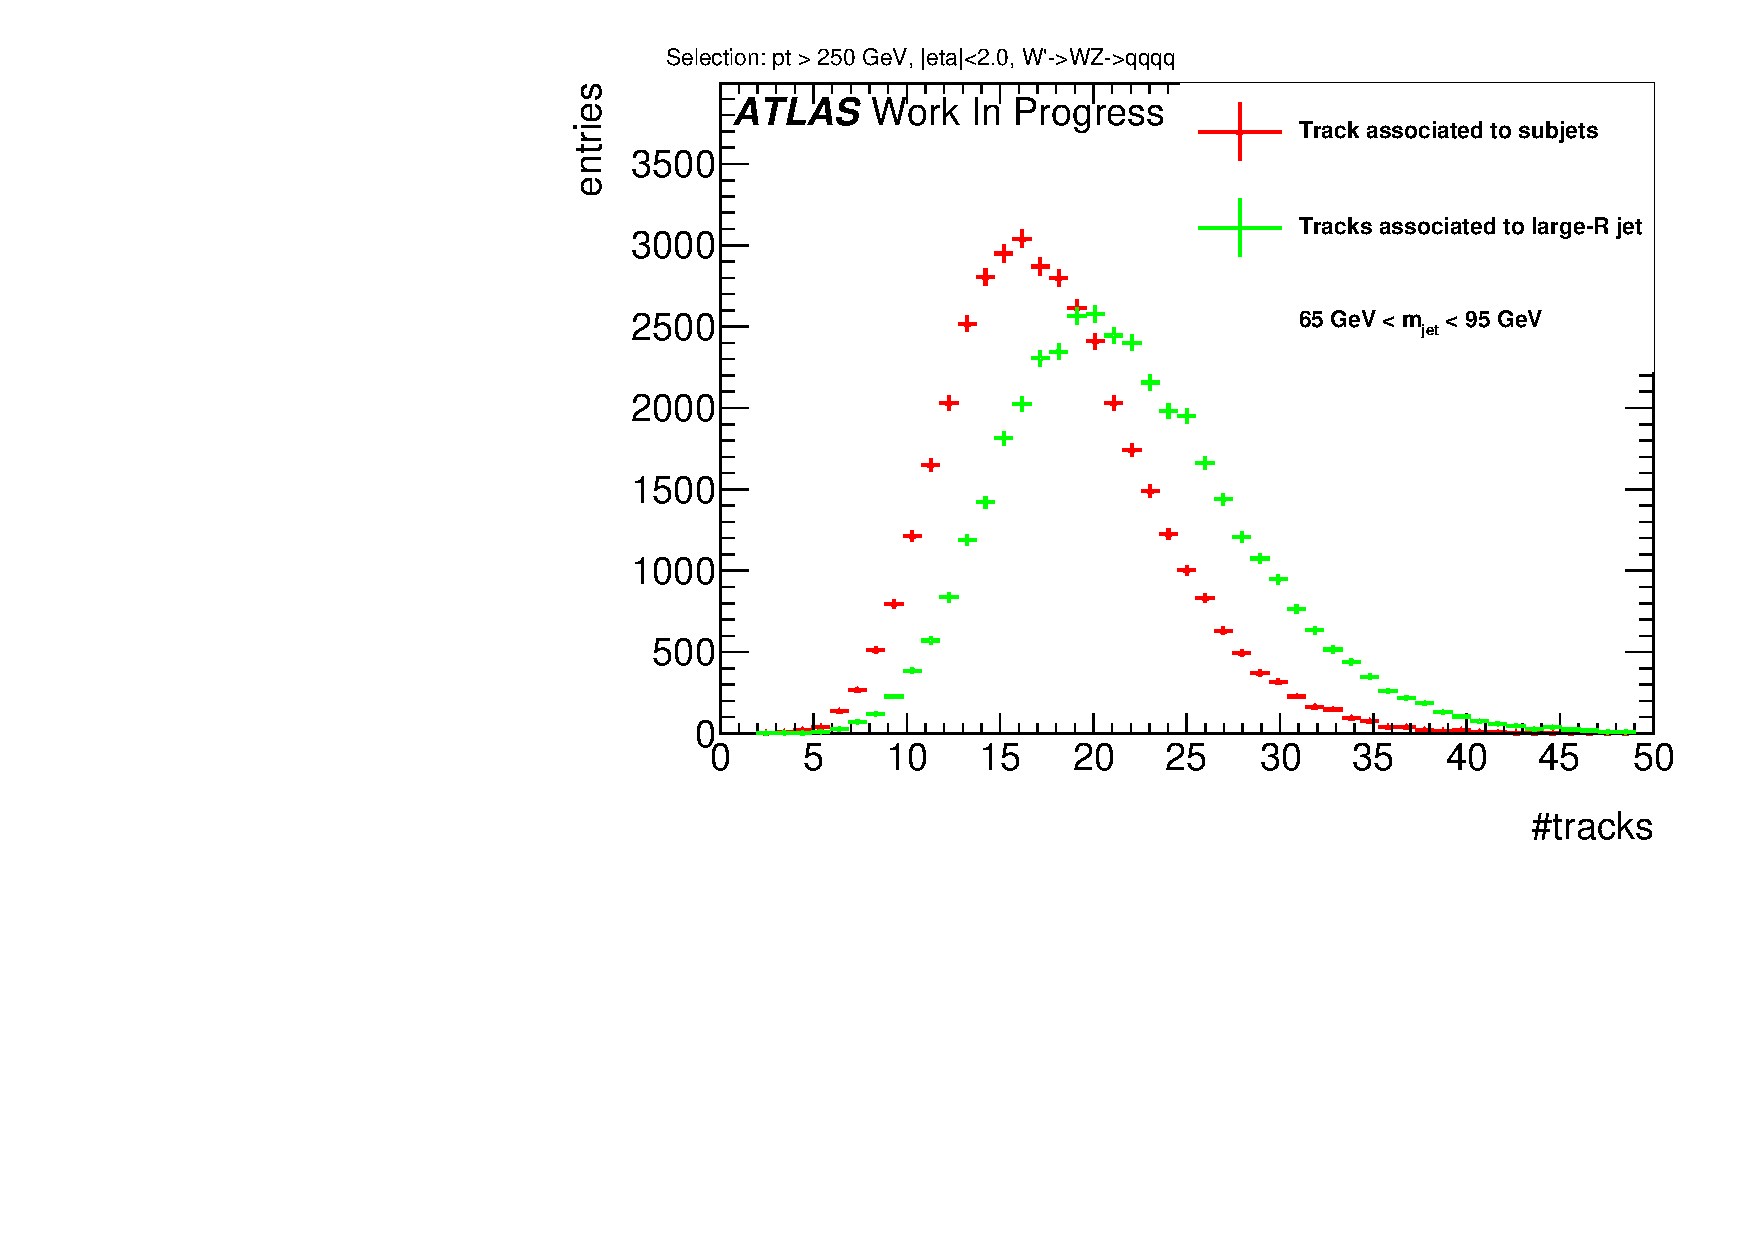
\includegraphics[width=0.45\textwidth]{sascha_input/plots/track_selection/h_customghost_number.pdf} \hspace{1mm}
	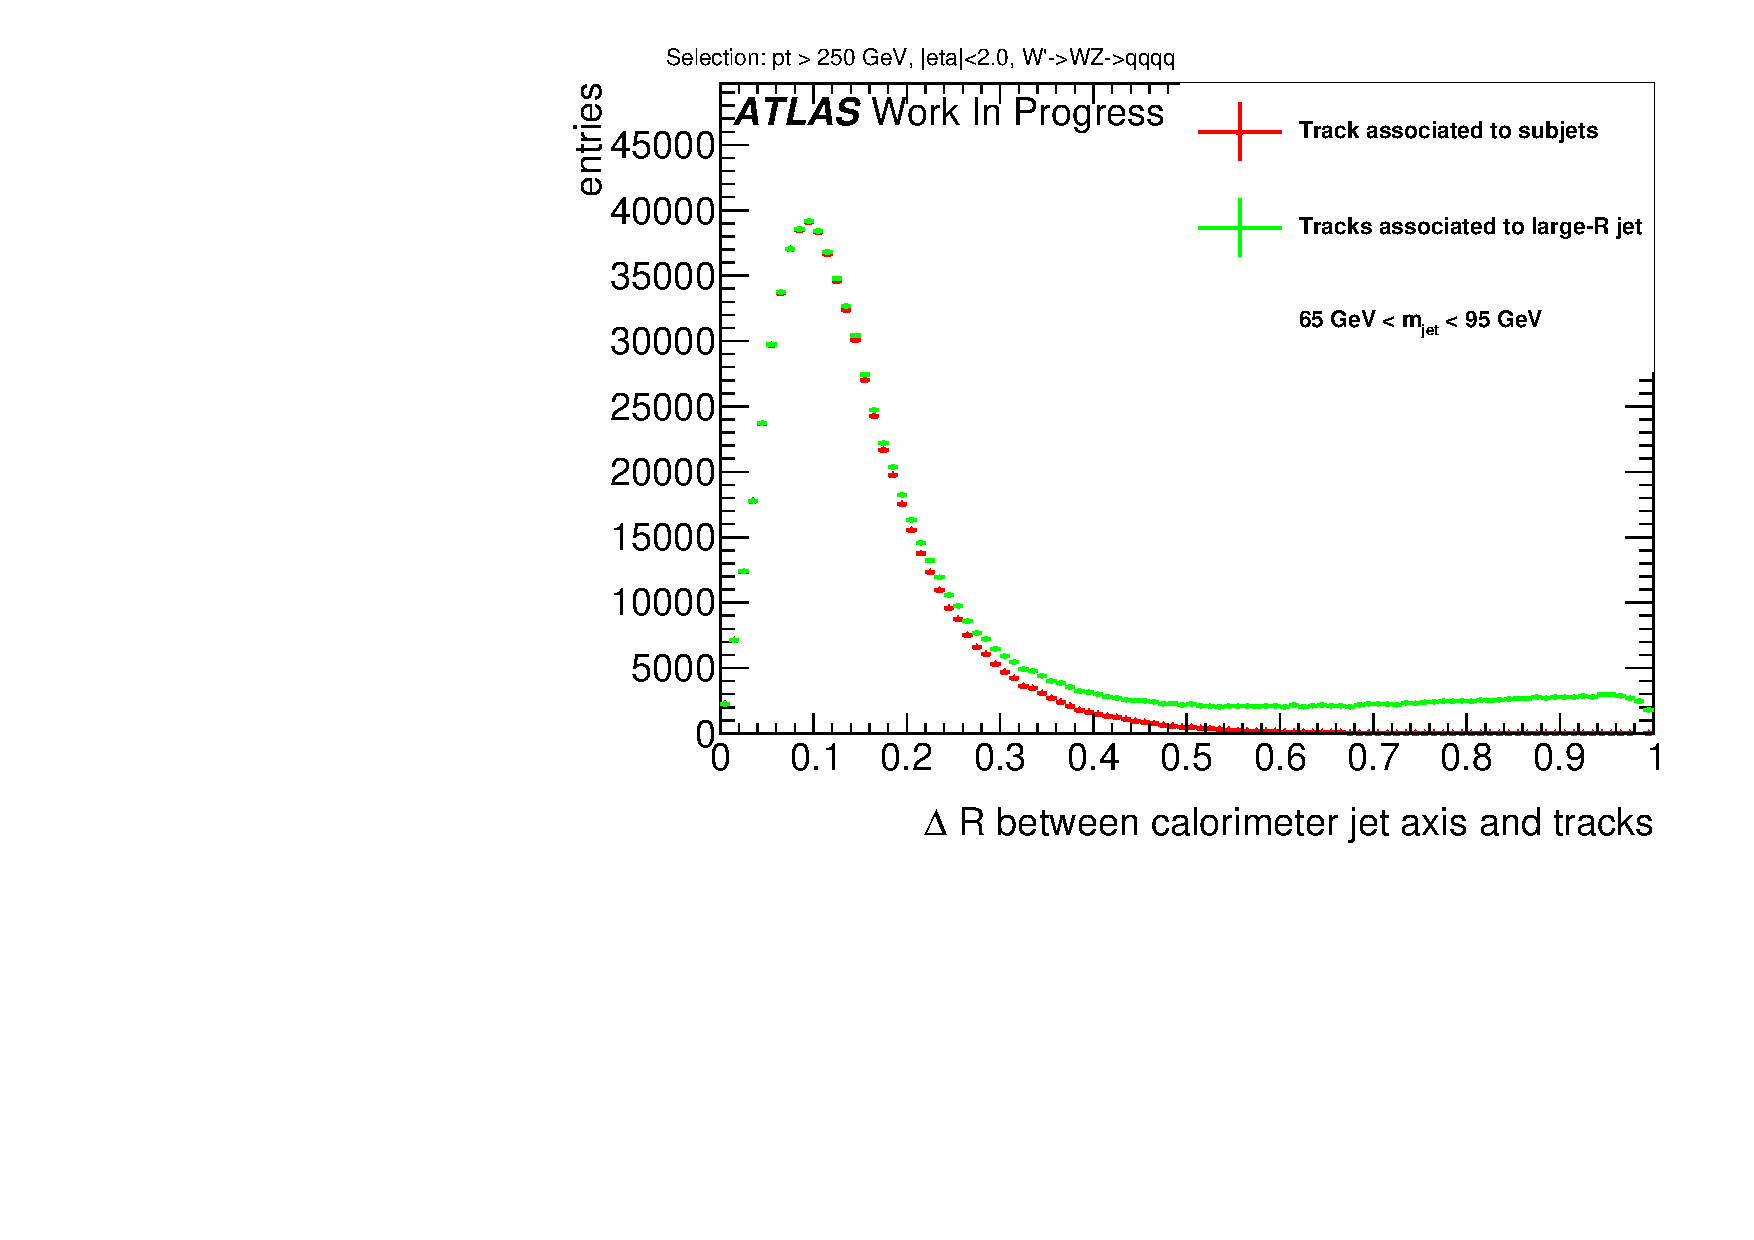
\includegraphics[width=0.45\textwidth]{sascha_input/plots/track_selection/h_customghost_dr.pdf}
\caption{\footnotesize{The number of tracks ghost associated to the large-R jet and to the subjets (left) and angular distance of associated tracks to the large-R calorimeter jet axis (right). Signal events were not reweighted at this step.}}\label{fig:delta_R}
\end{figure}


Figure \ref{fig:selection} shows the signal distributions of the C2/D2, and $\tau_{21}$, calculated with both selections of tracks for $W$ boson jets. The large $\Delta R$ to the jet axis of the differing tracks push the substructure variables to higher, more background like values. The broader distributions are a result of the variating nature of these tracks. C2 and D2 are more sensitive to tracks with a large $\Delta R$ to the jet axis, because the angular distance between all pairs and triples of tracks is considered, among tracks on possibly opposite sides of the large-R jet. The distances to $k_\mathrm{T}$-WTA axes used by $\tau_{21}$ are more robust against these scenarios.
\begin{figure}
	\centering
	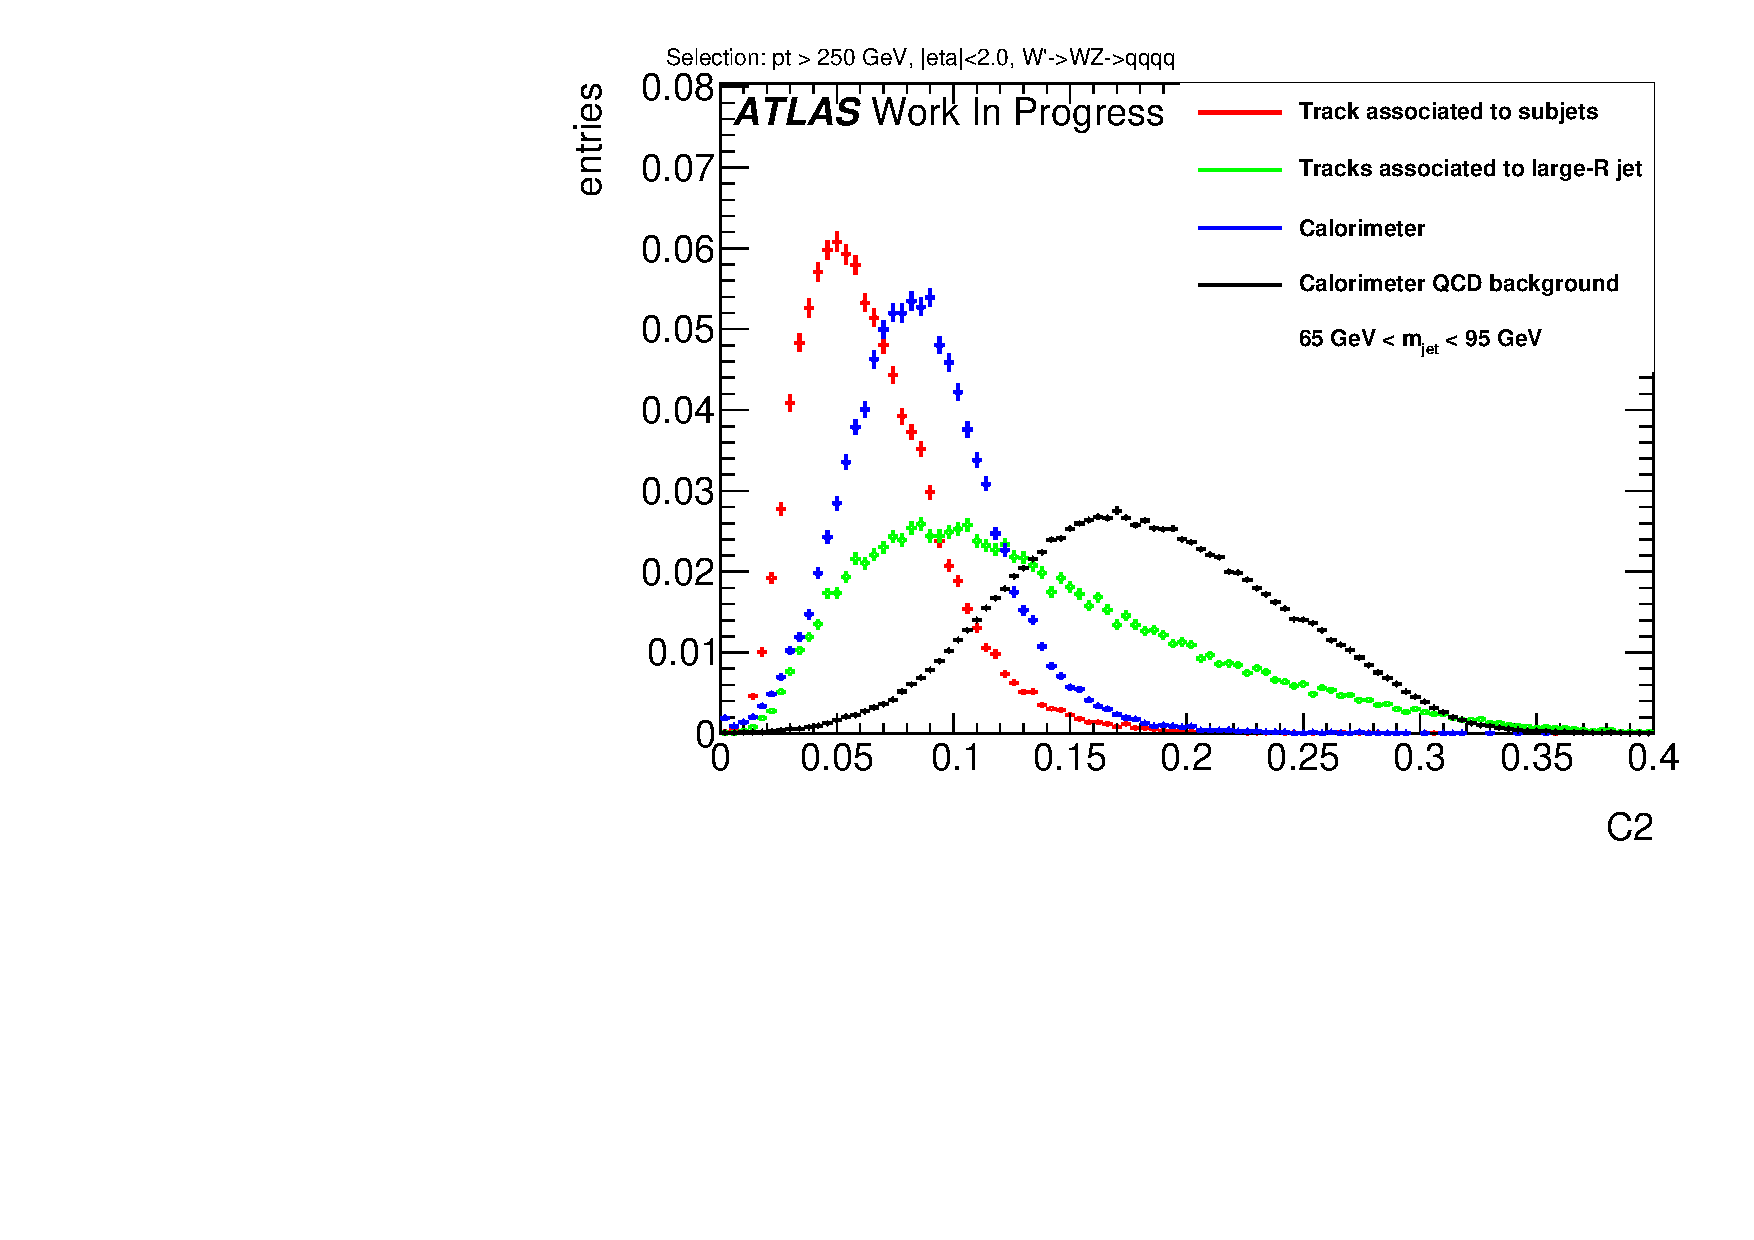
\includegraphics[width=0.3\textwidth]{sascha_input/plots/track_selection/h_ghost_sj_C2.pdf} 
	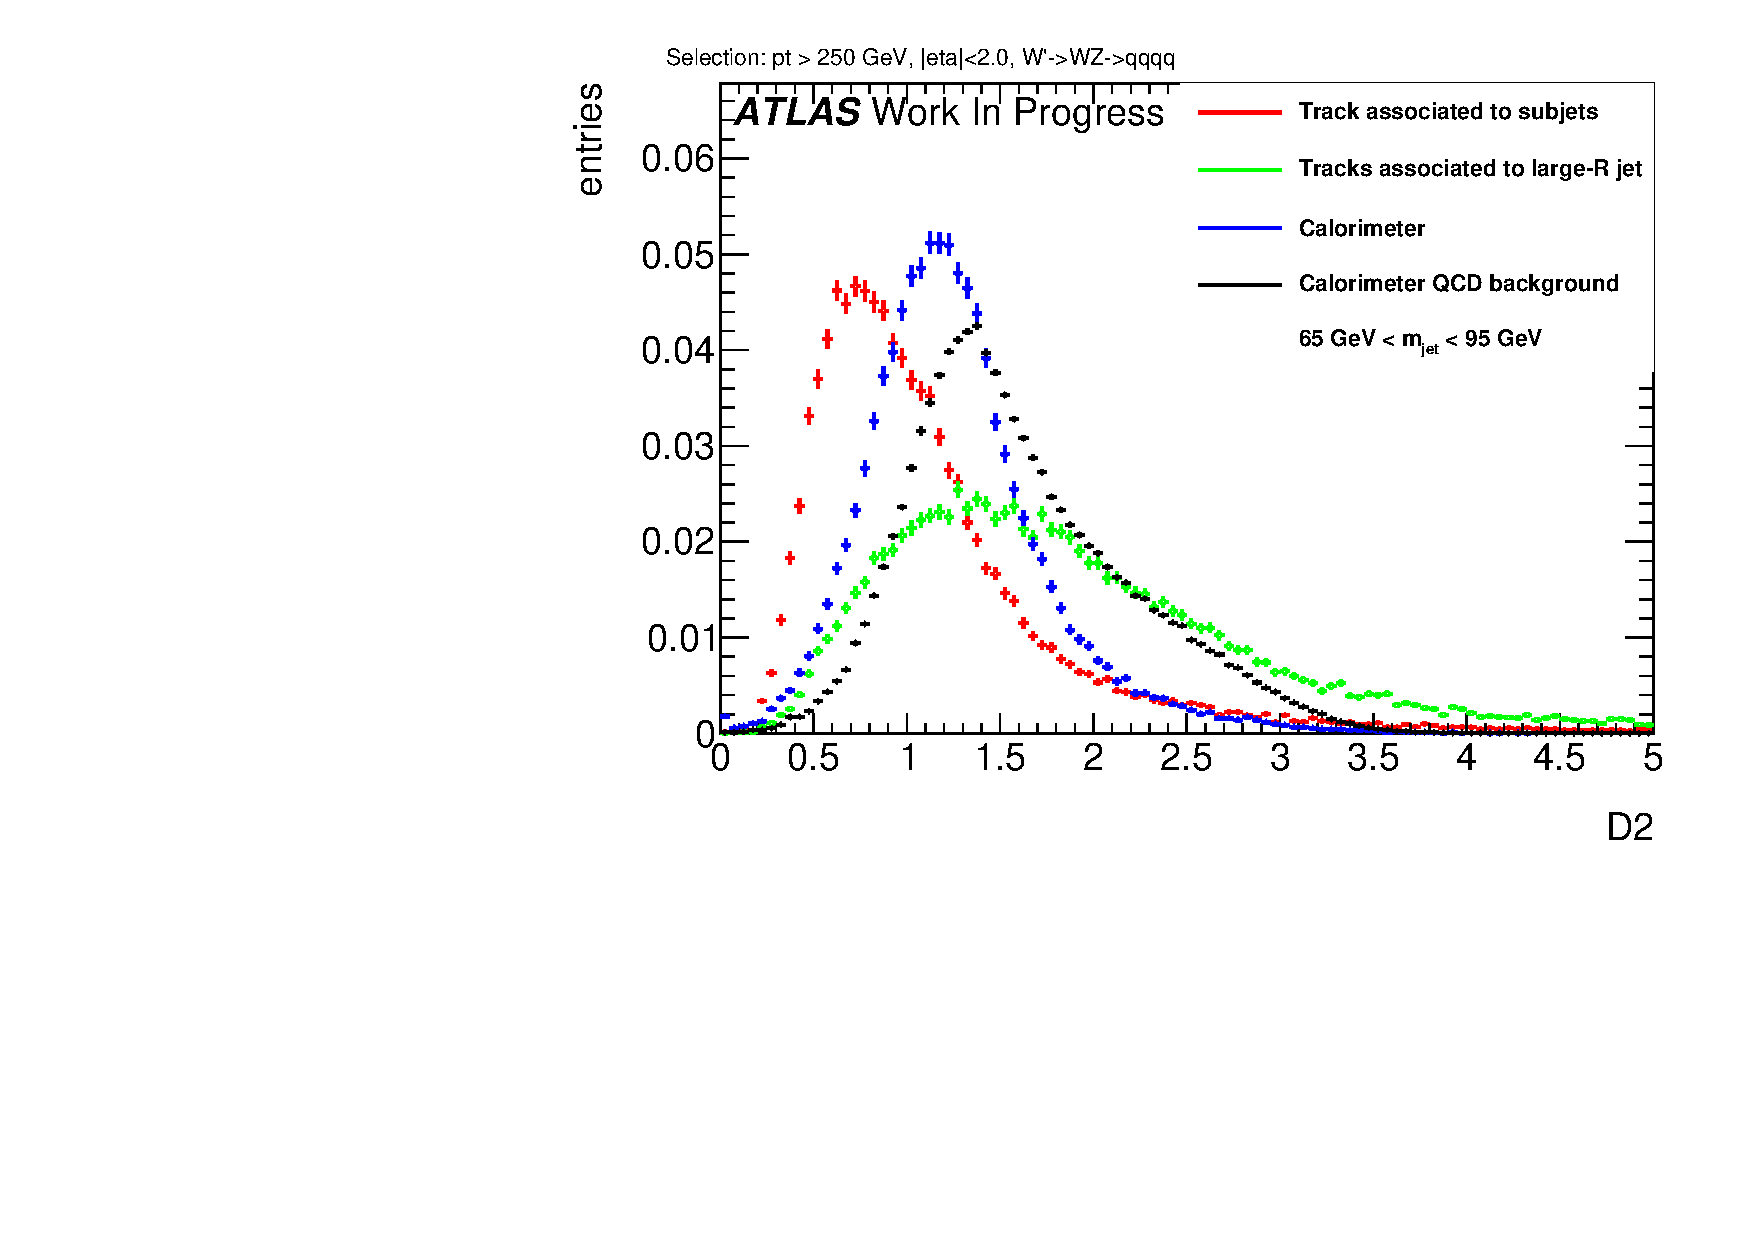
\includegraphics[width=0.3\textwidth]{sascha_input/plots/track_selection/h_ghost_sj_D2.pdf}
	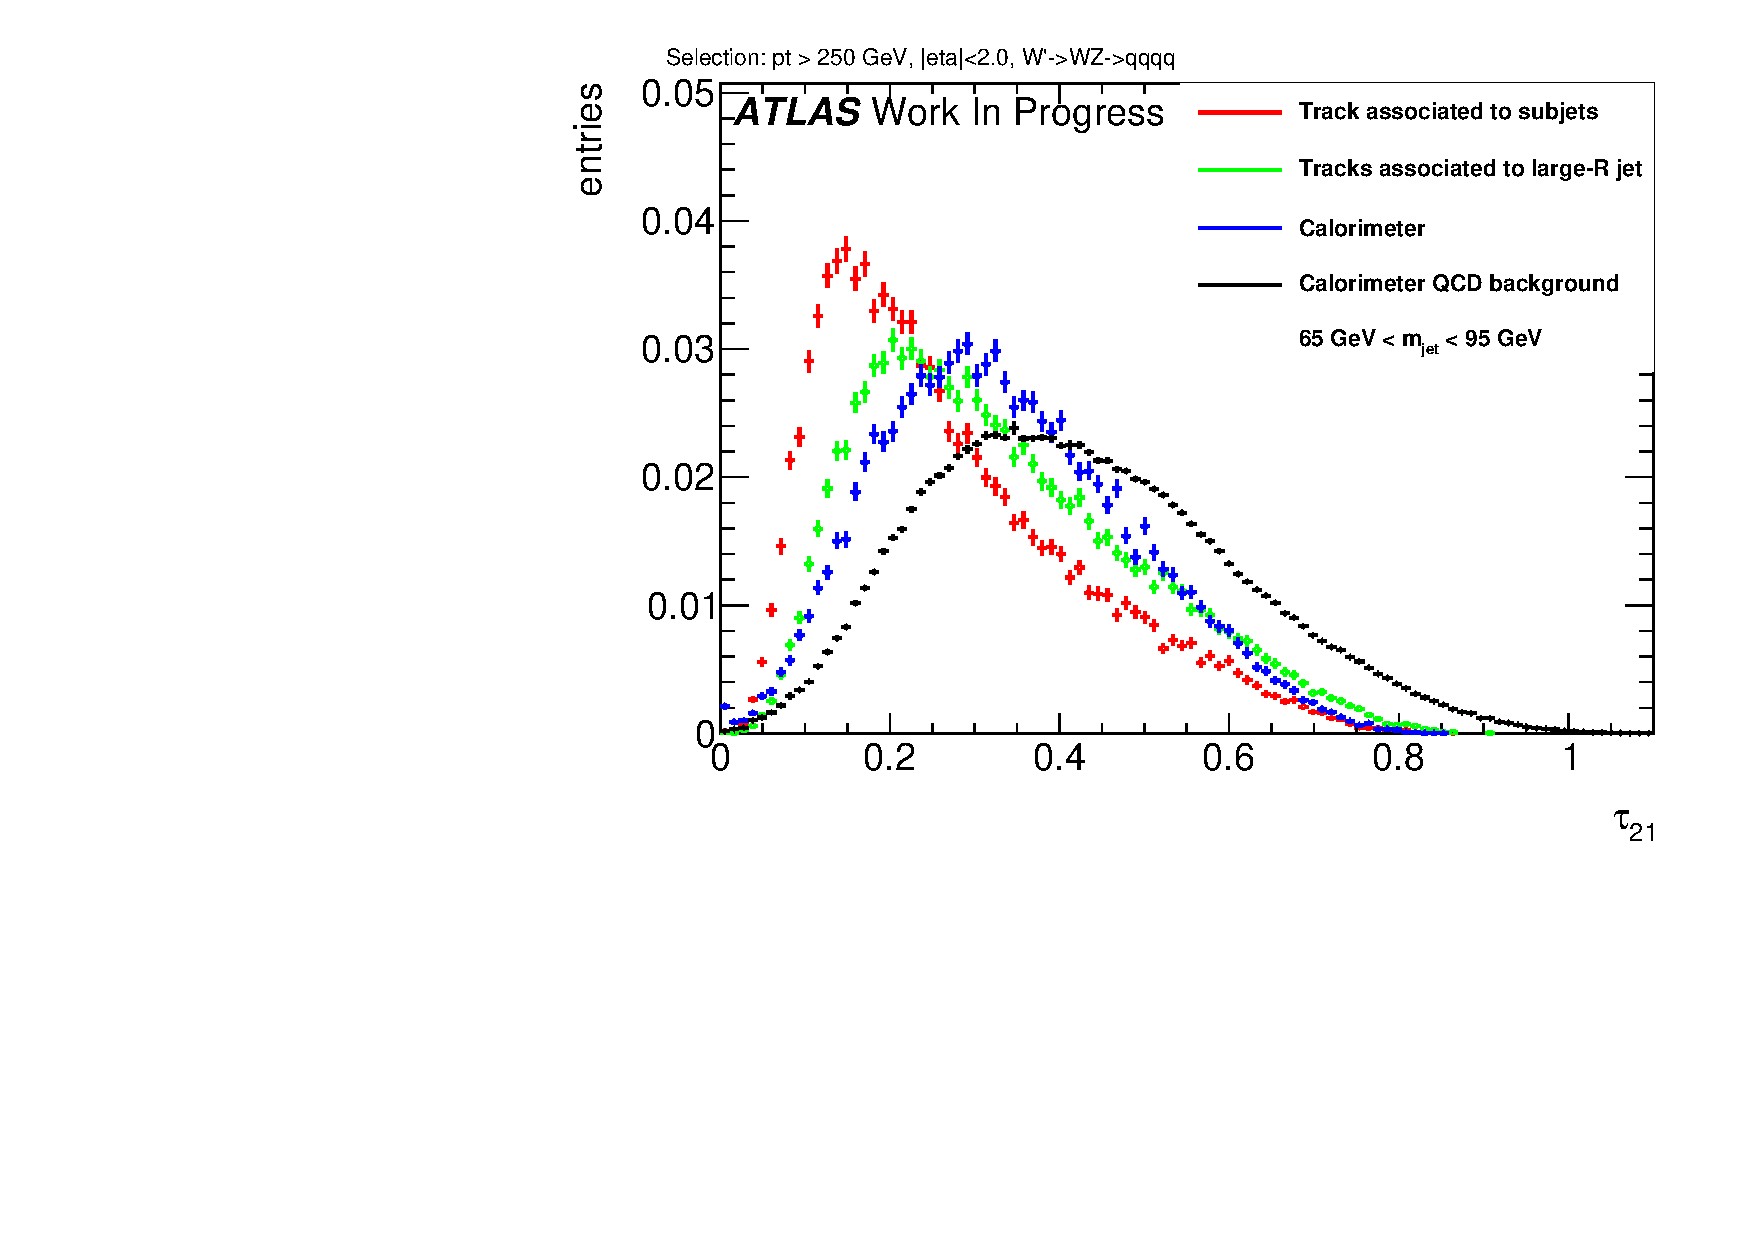
\includegraphics[width=0.3\textwidth]{sascha_input/plots/track_selection/h_ghost_sj_nSub21.pdf}
\caption{\footnotesize{Substructure variables (left) C2, (right) D2 and (below) $\tau_{21}$ calculated with calorimeter clusters as well as tracks associated to subjets and to the large-R jet. Signal events were not reweighted at this step.}}\label{fig:selection}
\end{figure}
For comparison, the signal and background distributions for the variables calculated with calorimeter clusters are shown as well. We expect that variables calculated with (assisted) tracks do not perform worse than cluster based pendants. In contrast to the jet mass, ratios of ECF(N,$\beta$) and $\tau_N$ are quite energy scale independent. They are found to not be as sensitive to the missing neutral fraction with un-assisted tracks, justifying the study of normal tracks next to TAS as input. 